% to compile this document use the following four commands: 
% pdflatex worms.tex
% bibtex worms.aux
% pdflatex worms.tex
% pdflatex worms.tex
\documentclass[12pt]{scrartcl}

% used packages
\usepackage{graphicx}
\usepackage{url}
\usepackage{listings}

% settings for listings
\lstset{language=Java}
\lstset{frame=single}
\lstset{framesep=10pt}
\lstset{basicstyle=\ttfamily}

% title, authors and date
\title{Oblig 2 \\ Creating a Domain Specific Language using the Eclipse Modelling Framework}
\author{Tobias Birmili, Florian Hagenauer, Kacper Surdy}

\date{07.05.2012}

\begin{document}

\maketitle

\tableofcontents

\section{Introduction}

This article is part of the second assignment for the course Modelbased System Development. The article discusses
how the three parts of the assignment have been solved. The basic task was to build a model for customer journeys,
make it possible to extract statistics out of customer journeys and finally the option to choose between three
additional tasks. It was possible to chose between a user-friendly editor, a graphical exporter or adding support
for multiple journeys. For this article the graphical export option was chosen.

Section \ref{section:model} describes how the model was built and discusses the different components. The second
section \ref{section:statistic} depicts which statistics were generated and Section \ref{section:export}
shows a solution for a graphical exporter which generates useful graphs. Finally, Section \ref{section:impl} shows
some details about the implementation and how we used the EMF tools.

\section{Creating a DSL metamodel with EMF} 
\label{section:model}

The first part of the work was to create a metamodel using the Eclipse Modelling Framework (EMF) for a customer
journey. A customer journey describes a collection of touchpoints a customer has with a product. Such a journey
usually consists of a reference which is the ideal way. After finalizing this journey some customer are asked
to take the journey and rate the different touchpoints and mybe add new ones. Every touchpoint should be rated
and if possible commented. For this metamodel some example journeys consisting of a reference journeys and four
different customer journeys which differ in some ways from the reference. 

\subsection{Domain Specific Language Metamodel}
The model itself consists of three main components. The first one is the \lstinline!JourneySet!. This component
includes the reference journey and a set of examples. A reference journey has to be set to allow comparison
between the example journeys and the reference. This component also has a method which allows the comparison
of the journeys to the reference journey. 

The second component is the \lstinline!Journey! which depicts the Customer journey itself. This journey consists of 
an ID, a more descriptive name, a date, the status and  an optional comment. If the ID of a journey is 
\lstinline!reference! then the journey is considered to be the reference journey. The model also contains some 
methods which allow to compare the journeys and generate statistics for a special journey or generate the graphical
representation. A more detailed description of this can be found in the Sections \ref{section:statistic} and
\ref{section:export}.

The last main component is called \lstinline!Touchpoint!. It describes the users interaction and experience during
a journey. Beside an ID, a name, a date and a comment it also has a type which describes if it is a generic or
and ad-hoc touchpoint, and evaluation where the customer votes how good the experience at the touchpoint was, a 
initiator for the touchpoint and finally a channel through which this touchpoint was experienced. The variables
channel, component, type, initiator and evaluation were done as enums. In that way they can be extended quite
easily by adding a new type to the enum and generate the new code.

Another part, which is important for \ref{section:statistic}, is the component \lstinline!JourneyDiff! which stores
the differences between the reference journey and the different example journeys.

\section{Making a transformation to extract statistics} 
\label{section:statistic}

The second task was to extend the model to generate statistics and print them in a convenient form. To represent
this generation in the model some methods were added to the \lstinline!JourneySet! and to the \lstinline!Journey!
components. The \lstinline!JourneySet! has the operation \lstinline!getComparedToExpected! to compare the example 
journeys from the set to the reference journey. The single journeys got methods which allow to extract single
statistics for the journey. These statistics are:
\begin{description}
	\item[Rating Statistic] These statistics scan the different rating types and allow to see how often each rating
	was given and the percentage of the total ratings.
	\item[Channel Statistics] These statistics cover the number of channels and percentage.
	\item[Initiator Statistics] How often an initiator invoked touchpoints can be found in this statistic.
	\item[Compare To Reference] This statistic shows how much the example journey differ from the given reference
	journey.
\end{description}

One part of the assignment was to print the statistics in a convenient and useful way. We choose to use the 
Markdown \footnote{\url{http://daringfireball.net/projects/markdown/}} to generate html files. Markdown allows
to write pretty simple statements to get well formatted text for html. Even the source code of Markdown is 
human readable and therefore useful. After generating the the markdown also a html website is built which allows
to see the statistics in a web-browser. With the choice of Markdown it is possible to generate a readable text
output and a very nice html output.

\section{Graphical Export} 
\label{section:export}

The last part of the assignment was to choose between different extensions for the metamodel. In this article
the graphical export feature was chosen. The task was to generate a graphical representation of the customer
journeys to make them more easy to understand. The choice in this article fell to Graphviz 
\footnote{\url{http://graphviz.org/}} a visualization tool that allows to print graphs in a convenient way.
The metamodel was extended with the operation \lstinline!getGraphviz! inside of \lstinline!JourneySet! and
\lstinline!Journey!. The basic idea can be seen in Figure \ref{figure:sample_figure}.

\begin{figure}[hbtp]
	\centering
	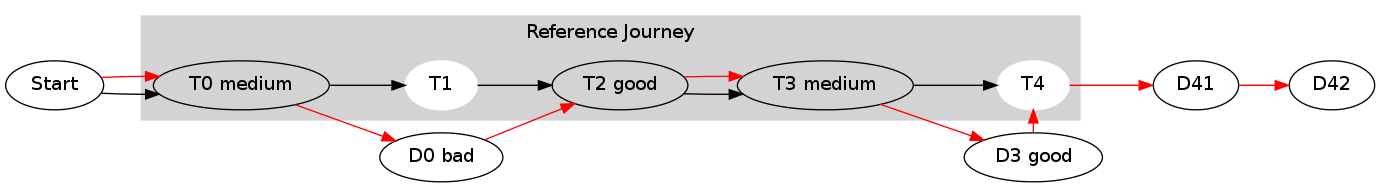
\includegraphics[scale=0.35]{img/sample_journey1.png}
	\caption{The basic idea for the visualization}
	\label{figure:sample_figure}
\end{figure}

The basic idea is to have the reference journey, here depicted in the grey box and the black arrows, and the 
example journey, which has red arrows in the example. It should be easy to spot the difference between the
reference and the example journey. Also the ratings are directly included into the graph.


\section{Implementation Details}
\label{section:impl}

In this section some details about the implementation and the general project can be found. Figure 
\ref{figure:projects} shows the different projects for the assignment.

\begin{figure}[hbtp]
	\centering
	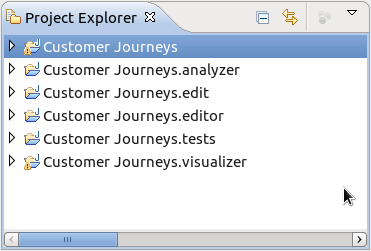
\includegraphics[scale=0.5]{img/projectexplorer.png}
	\caption{The different Eclipse projects of the assignment}
	\label{figure:projects}
\end{figure}

The project Customer Journey is the main project which contains the model and the generated code. The three
projects .edit .editor and .tests are generated by the model. The .editor was used to define the example and
the reference journeys. The project .analyzer contains the source code to load a customer journey set and
return the analysis. Finally, the .visualizer project is responsible for visualizing the customer journeys as 
described in Section \ref{section:export}.

For version control a github repository was used\footnote{\url{https://github.com/floxyz/INF5120}}.

\end{document}